%-----------------------------------------------------------------------------80
% CONTENT
%-----------------------------------------------------------------------------80
\subsection{Entorno de desarrollo Windows}


\begin{frame}[fragile]{Instalación de editor de código}
  \textbf{VS Code en Windows}
  \begin{itemize}
    \item Descargar el instalador desde \url{https://code.visualstudio.com/download}
  \end{itemize}  
    \begin{figure}
      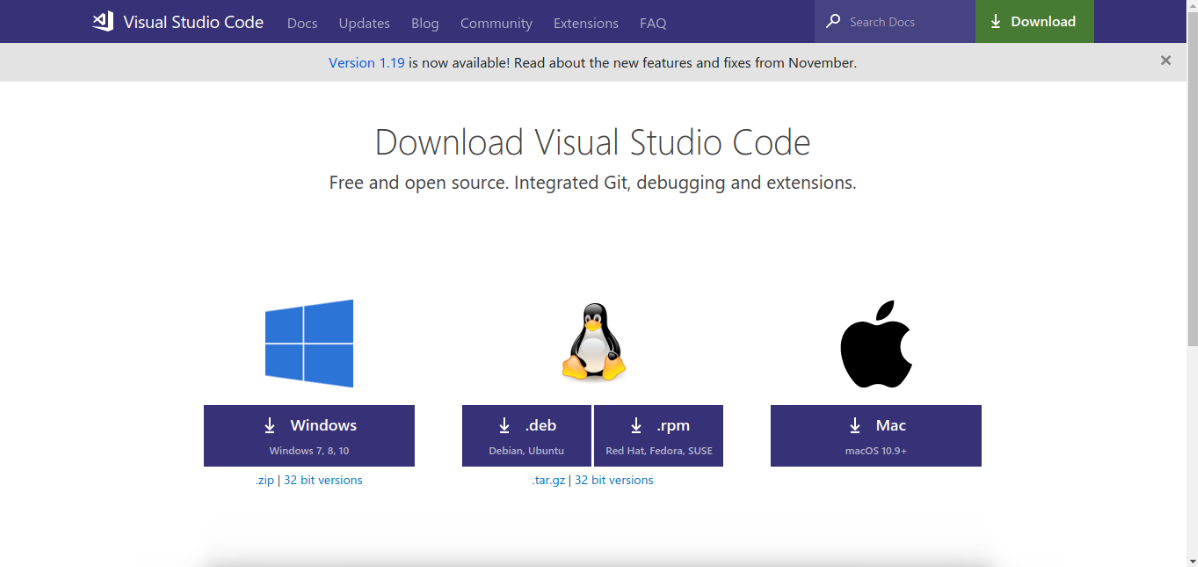
\includegraphics[width=0.9\textwidth]{./resources/1.png}
      \caption*{Página oficial de Visual Studio Code}
    \end{figure}
\end{frame}


\begin{frame}[fragile]{Instalación de editor de código}
  \textbf{VS Code en Windows}
   \begin{itemize}
    \item Iniciar el instalador y seguir los siguientes pasos:
   \end{itemize} 
   \begin{figure}
      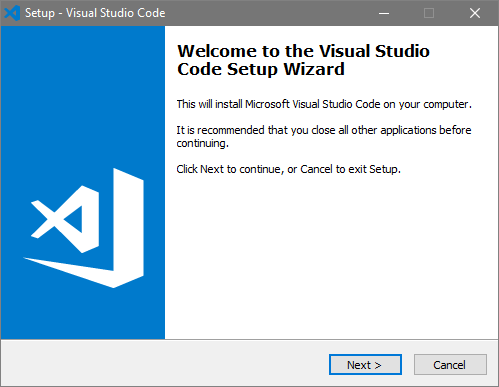
\includegraphics[width=0.7\textwidth]{./resources/VSCODE_Step_01.PNG}
   \end{figure}
\end{frame}

\begin{frame}[fragile]{Instalación de editor de código}
  \textbf{VS Code en Windows}
   \begin{figure}
     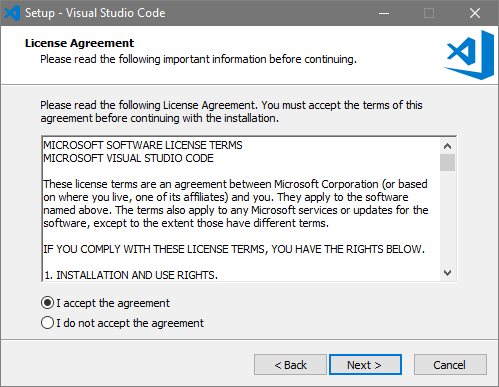
\includegraphics[width=0.8\textwidth]{./resources/VSCODE_Step_02.PNG}
   \end{figure}
\end{frame}

\begin{frame}[fragile]{Instalación de editor de código}
  \textbf{VS Code en Windows}
   \begin{figure}
     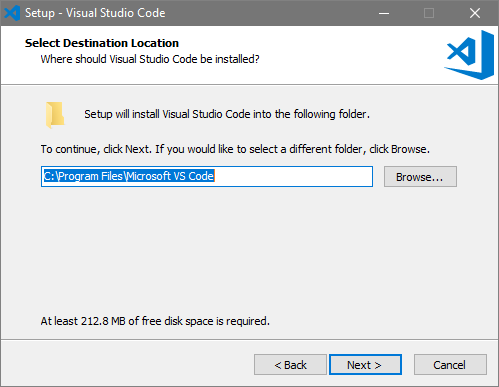
\includegraphics[width=0.8\textwidth]{./resources/VSCODE_Step_03.PNG}
   \end{figure}
\end{frame}

\begin{frame}[fragile]{Instalación de editor de código}
  \textbf{VS Code en Windows}
   \begin{figure}
     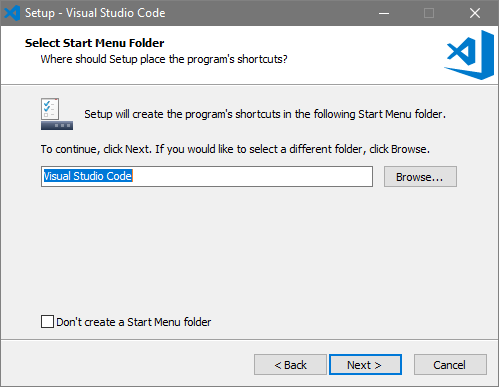
\includegraphics[width=0.8\textwidth]{./resources/VSCODE_Step_04.PNG}
   \end{figure}
\end{frame}

\begin{frame}[fragile]{Instalación de editor de código}
  \textbf{VS Code en Windows}
   \begin{figure}
     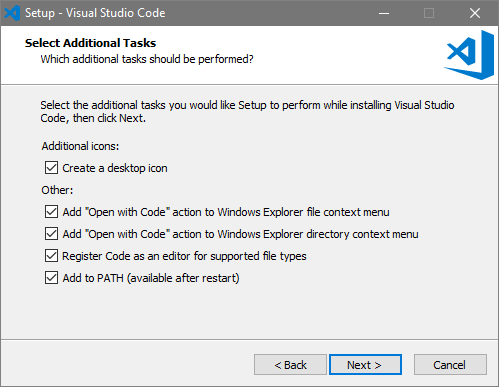
\includegraphics[width=0.8\textwidth]{./resources/VSCODE_Step_05.PNG}
   \end{figure}
\end{frame}

\begin{frame}[fragile]{Instalación de editor de código}
  \textbf{VS Code en Windows}
   \begin{figure}
     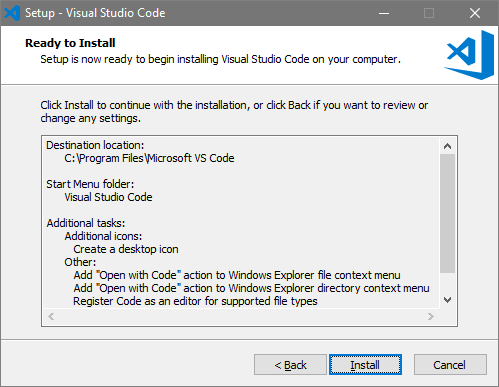
\includegraphics[width=0.8\textwidth]{./resources/VSCODE_Step_06.PNG}
   \end{figure}
\end{frame}

\begin{frame}[fragile]{Instalación de editor de código}
  \textbf{VS Code en Windows}
   \begin{figure}
     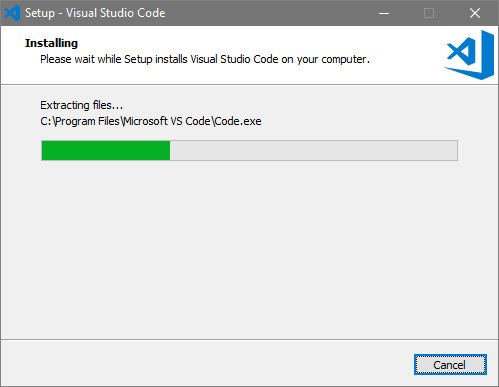
\includegraphics[width=0.8\textwidth]{./resources/VSCODE_Step_07.PNG}
   \end{figure}
\end{frame}

\begin{frame}[fragile]{Instalación de editor de código}
  \textbf{VS Code en Windows}
   \begin{figure}
     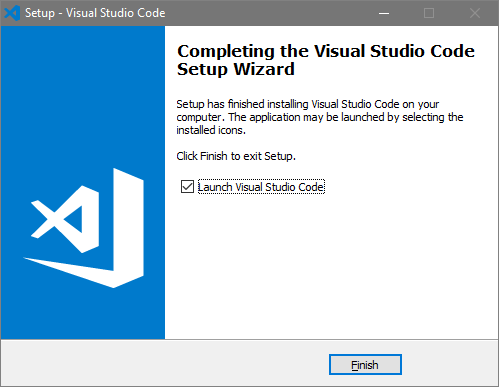
\includegraphics[width=0.8\textwidth]{./resources/VSCODE_Step_08.PNG}
   \end{figure}
\end{frame}

\begin{frame}[fragile]{Instalación de compilador y debuger}
 \textbf{Instalación del compilador TDM-GCC}
 \begin{itemize}[<+(1)->]
  \item Descargar el paquete TDM-GCC según la versión de windows (32-64 bits) en \url{http://tdm-gcc.tdragon.net/}
  \item Iniciar el instalador y seguir los siguientes pasos:
 \end{itemize}
 \onslide<3->   \begin{figure}
                    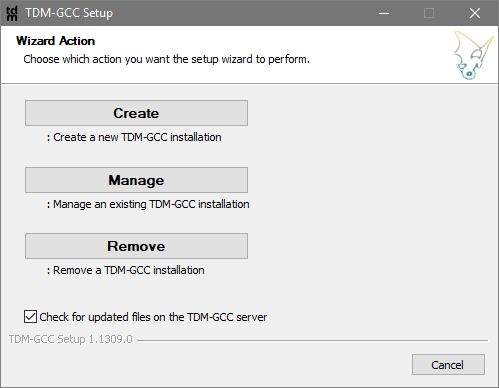
\includegraphics[width=0.65\textwidth]{./resources/TDMGCC_Step_01.PNG}
                \end{figure}
\end{frame}

\begin{frame}[fragile]{Instalación de compilador y debuger}
 \textbf{Instalación del compilador TDM-GCC}
  \begin{figure}
      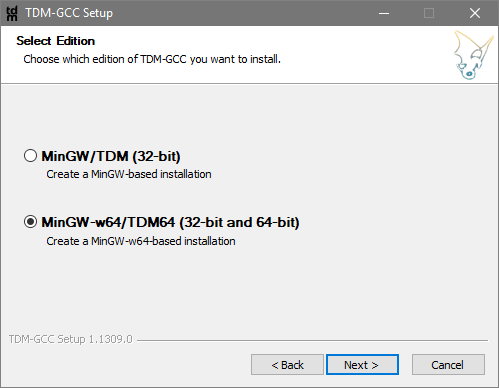
\includegraphics[width=0.8\textwidth]{./resources/TDMGCC_Step_02.PNG}
  \end{figure}
\end{frame}

\begin{frame}[fragile]{Instalación de compilador y debuger}
 \textbf{Instalación del compilador TDM-GCC}
  \begin{figure}
      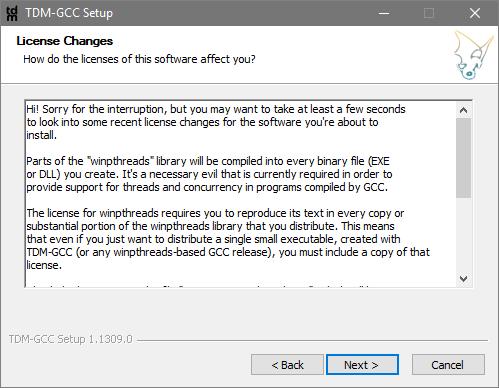
\includegraphics[width=0.8\textwidth]{./resources/TDMGCC_Step_03.PNG}
  \end{figure}
\end{frame}

\begin{frame}[fragile]{Instalación de compilador y debuger}
 \textbf{Instalación del compilador TDM-GCC}
  \begin{figure}
      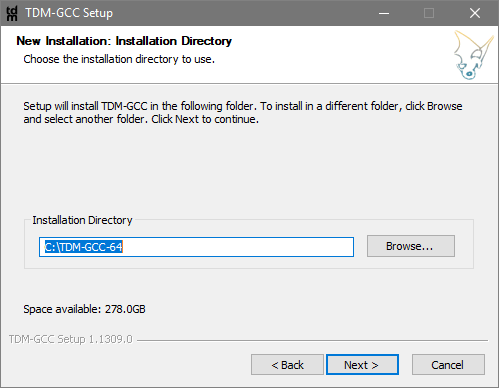
\includegraphics[width=0.8\textwidth]{./resources/TDMGCC_Step_04.PNG}
  \end{figure}
\end{frame}

\begin{frame}[fragile]{Instalación de compilador y debuger}
 \textbf{Instalación del compilador TDM-GCC}
  \begin{figure}
      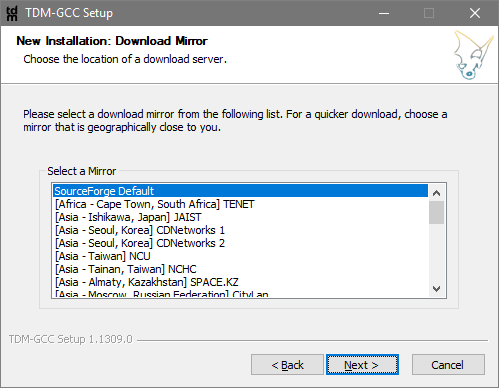
\includegraphics[width=0.8\textwidth]{./resources/TDMGCC_Step_05.PNG}
  \end{figure}
\end{frame}

\begin{frame}[fragile]{Instalación de compilador y debuger}
 \textbf{Instalación del compilador TDM-GCC}
  \begin{figure}
      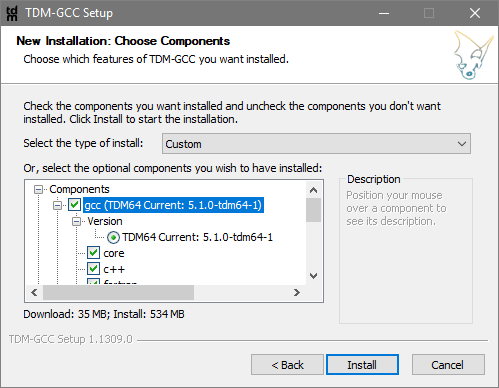
\includegraphics[width=0.8\textwidth]{./resources/TDMGCC_Step_06.PNG}
  \end{figure}
\end{frame}

\begin{frame}[fragile]{Instalación de compilador y debuger}
 \textbf{Instalación del compilador TDM-GCC}
  \begin{figure}
      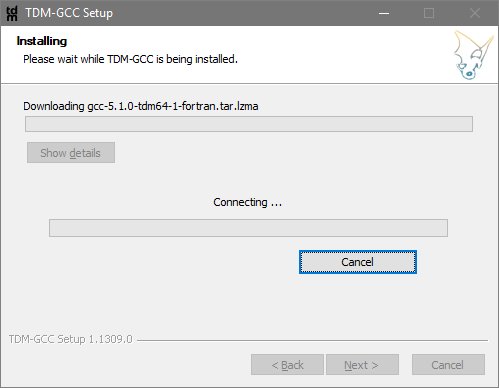
\includegraphics[width=0.8\textwidth]{./resources/TDMGCC_Step_07.PNG}
  \end{figure}
\end{frame}

\begin{frame}[fragile]{Instalación de compilador y debuger}
 \textbf{Instalación del compilador TDM-GCC}
  \begin{figure}
      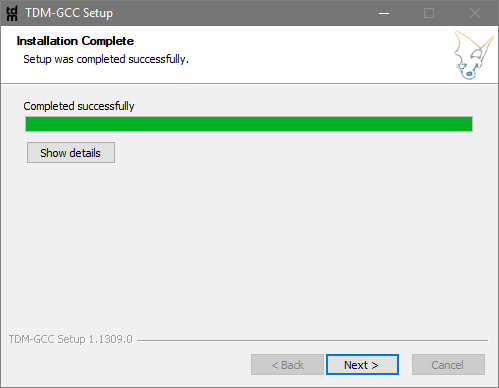
\includegraphics[width=0.8\textwidth]{./resources/TDMGCC_Step_08.PNG}
  \end{figure}
\end{frame}

\begin{frame}[fragile]{Instalación de compilador y debuger}
 \textbf{Instalación del compilador TDM-GCC}
  \begin{figure}
      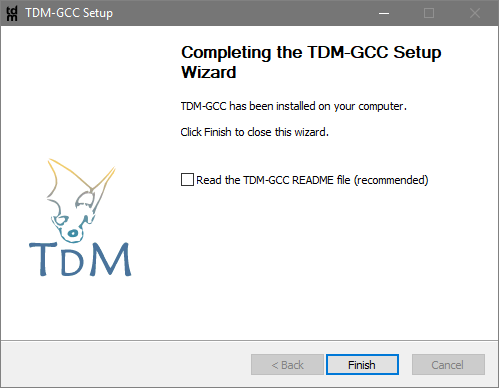
\includegraphics[width=0.8\textwidth]{./resources/TDMGCC_Step_09.PNG}
  \end{figure}
\end{frame}

